\documentclass[11pt]{article}
\usepackage[a4paper,margin=1in]{geometry}
\usepackage{amsmath,amssymb,amsthm}
\usepackage{graphicx,float,microtype,booktabs,array,xcolor}
\usepackage[colorlinks=true,linkcolor=blue!55!black,urlcolor=blue!60!black]{hyperref}
\newtheorem{theorem}{Theorem}
\newtheorem{lemma}[theorem]{Lemma}
\newtheorem{remark}[theorem]{Remark}
\newcommand{\C}{\mathbb C}
\newcommand{\D}{\mathbb D}
\newcommand{\Sph}{\mathbb S}
\newcommand{\J}{\mathcal J}
\newcommand{\Rad}{\mathcal R_c}
\newcommand{\Icp}{\mathrm I_{C,p}}
\newcommand{\Idp}{\mathrm I_{\D,p}}
\newcommand{\GL}{\mathrm{GL}}
\newcommand{\Gam}{\Gamma}
\title{Complex $L_p$-Intersection Bodies:\\Uniform Convexity Near Hermitian Ellipsoids}
\author{Automated mathematics run \texttt{fa\_banach\_001}\\Lane 0 --- candidate partial result}
\date{11 August 2026}
\begin{document}
\maketitle

\begin{center}
\fbox{\parbox{0.91\textwidth}{\textbf{Status.}
Partial answer to the open convexity question for $-2<p<-1$.
For each complex dimension, a single $C^2$ neighborhood of the Hermitian
ellipsoids works simultaneously for every exponent in the missing interval
and every admissible planar body $C$.  The proof is qualitative but uniform.
It does not settle arbitrary balanced convex bodies.}}
\end{center}

\section{The source question}

Ellmeyer--Hofst\"atter define complex $L_p$-intersection bodies by
\[
 \rho_{\Icp K}(u)^{-p}=\int_K h_{Cu}(x)^p\,dx,
 \qquad -2<p<0,
\]
where $C\subset\C$ contains the origin in its interior.  For an
$\Sph^1$-invariant convex $K\subset\C^n$, they prove convexity when
$p\ge -1$ and pseudoconvexity when $-2<p<-1$, and explicitly ask whether the
latter conclusion can be strengthened.

\begin{figure}[H]
\centering
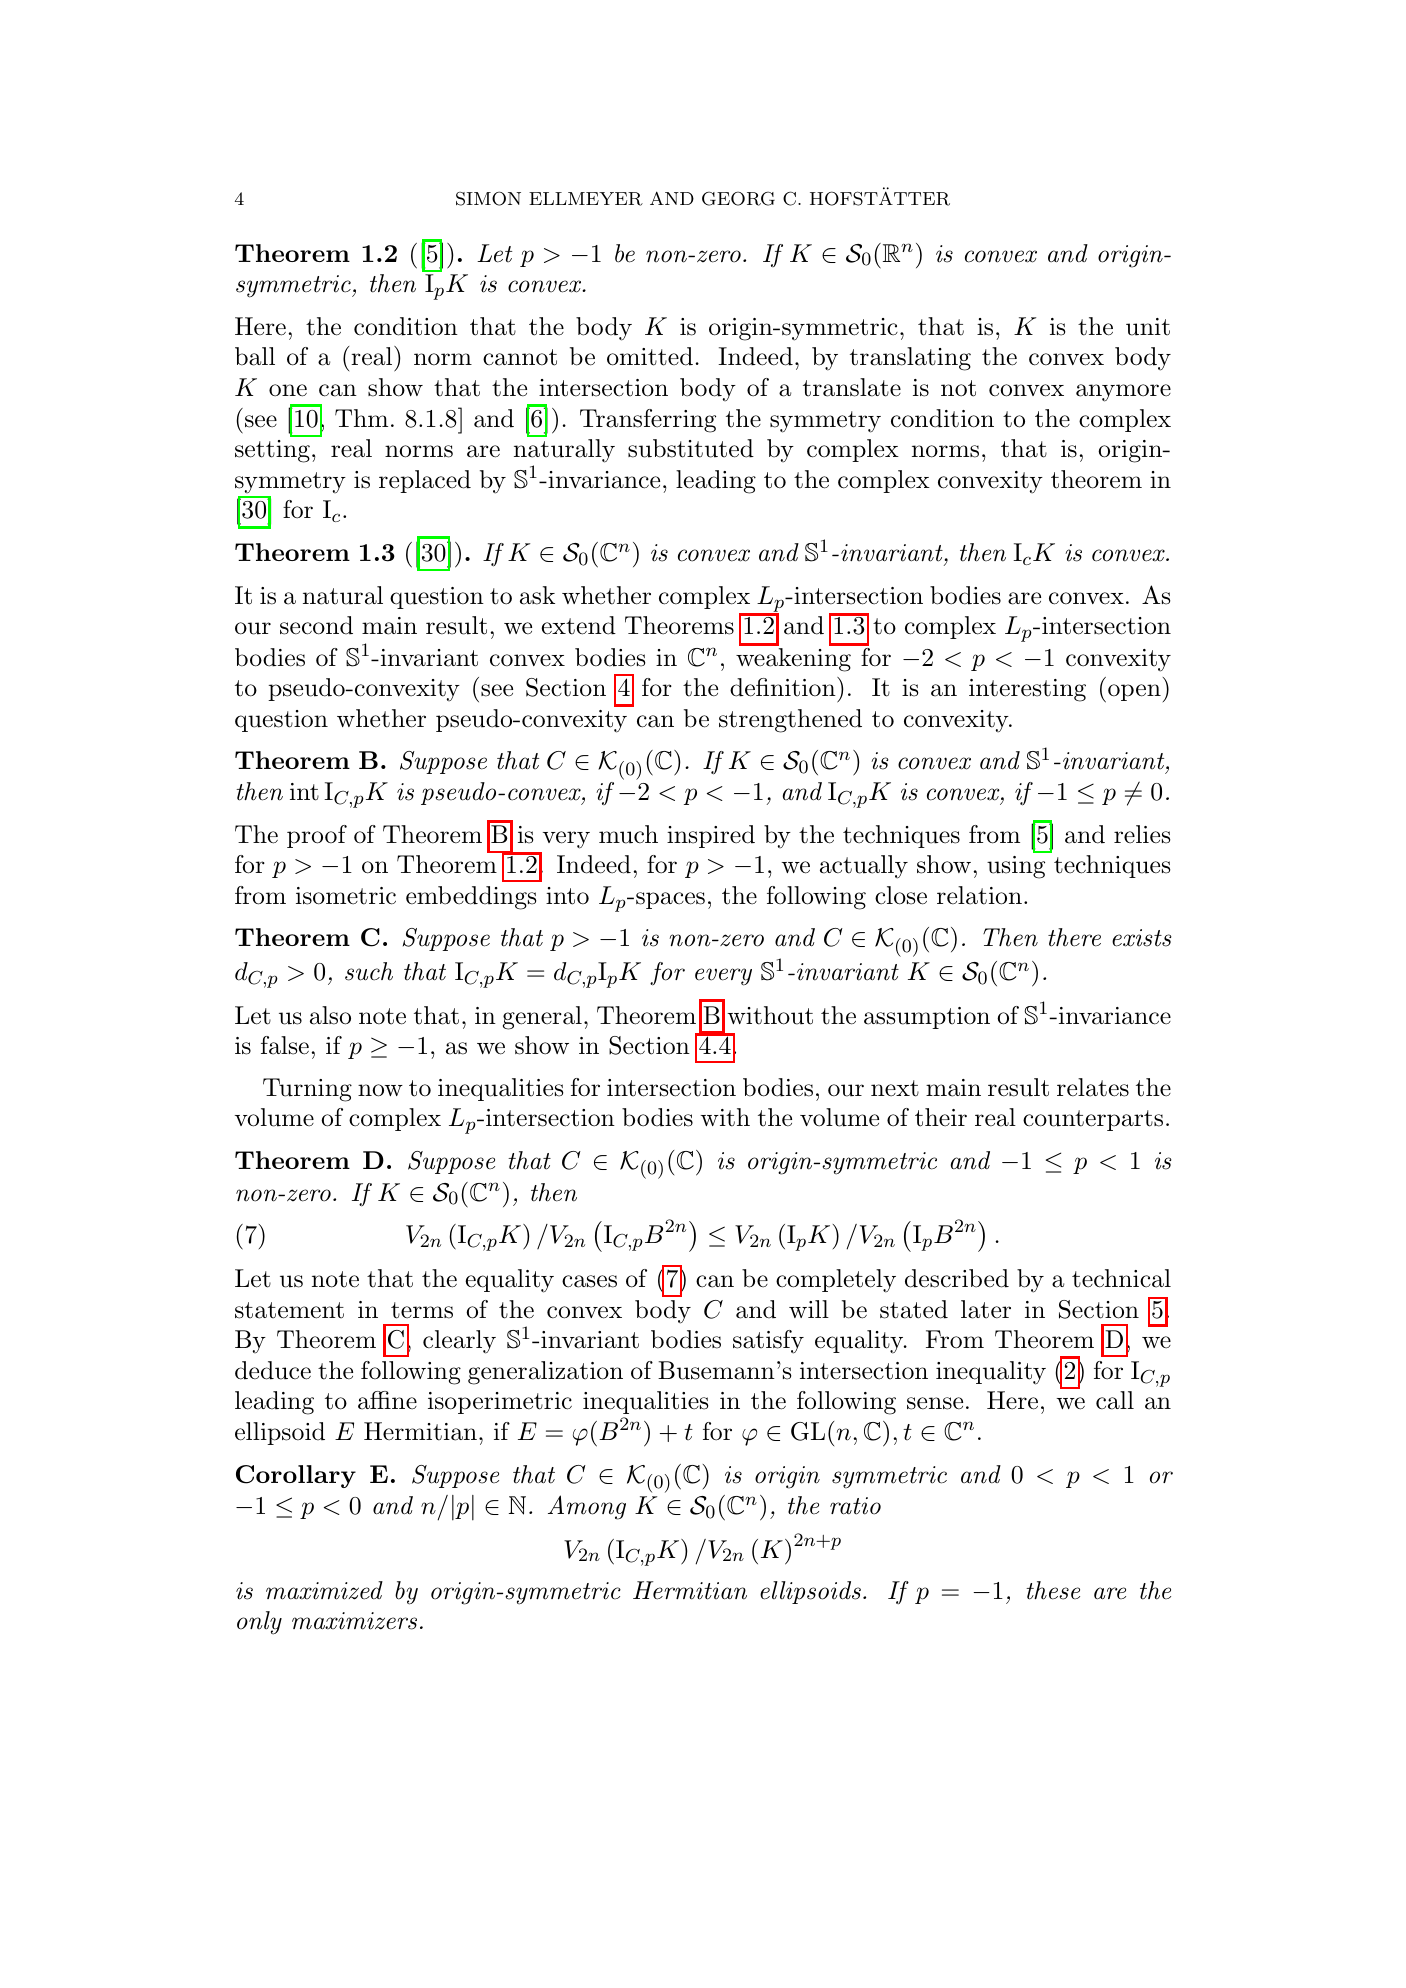
\includegraphics[width=0.91\textwidth,height=0.69\textheight,keepaspectratio]{figures/source_question-page4.png}
\caption{Compiled source page 4: the open convexity question and Theorem B.}
\end{figure}

For balanced data the source also proves that replacing $C$ by the unit disk
only changes the output by a homothety.  In the disk case, putting $q=-p$,
the reciprocal radial function is, up to a constant,
\[
 N_q(u)=\left(\int_K |x\mathbin{\cdot}u|^{-q}\,dx\right)^{-1/q},
 \qquad 1<q<2.                                                    \tag{1.1}
\]
Thus the full question asks whether (1.1) is always a complex norm.

\section{Statement of the partial result}

Use the covariant $C^2$ norm on the unit sphere.  A body is
\emph{$C^2$-close to a Hermitian ellipsoid} if some complex linear image has a
$C^2$ radial function close to one.

\begin{theorem}[one neighborhood for the whole missing interval]\label{thm:main}
For every $n\ge2$ there is $\varepsilon_n>0$ with the following property.
Let $K\subset\C^n$ be an $\Sph^1$-invariant convex body with a $C^2$ radial
function.  Suppose that for some $\Theta\in\GL(n,\C)$,
\[
 \bigl\|\rho_{\Theta K}-1\bigr\|_{C^2(\Sph^{2n-1})}<\varepsilon_n. \tag{2.1}
\]
Then $\Icp K$ is a strictly convex body for every
\[
 C\in\mathcal K_{(0)}(\C),\qquad -2<p<-1.                          \tag{2.2}
\]
The same $\varepsilon_n$ works simultaneously for all $p$ and all $C$ in
\textup{(2.2)}.
\end{theorem}

The input convexity assumption is included to match the source question.  In
fact, the proof only needs a positive balanced $C^2$ radial function satisfying
(2.1).

\section{A \texorpdfstring{$C^2$}{C2} endpoint lemma}

For $p>-2$ and $f\in C(\Sph^{2n-1})$, set
\[
 (T_pf)(u)=\frac1{\Gam(p+2)}
 \int_{\Sph^{2n-1}} |v\mathbin{\cdot}u|^p f(v)\,dv.                \tag{3.1}
\]
At $p=-2$, define $T_{-2}=c_n\Rad$, where $\Rad f(u)$ is the integral of
$f$ over the complex equator $\{v:v\cdot u=0\}$ and $c_n>0$ is the endpoint
constant.  Its exact value will not matter.

\begin{lemma}[$C^2$ strengthening of endpoint convergence]\label{lem:c2}
The map
\[
 [-2,-1]\times C^2(\Sph^{2n-1})\longrightarrow C^2(\Sph^{2n-1}),
 \qquad (p,f)\longmapsto T_pf,                                    \tag{3.2}
\]
is continuous.
\end{lemma}

\begin{proof}
The source proves the $C^0$ convergence $T_pf\to c_n\Rad f$ as
$p\downarrow-2$, including the version in which $f=f_p$ converges uniformly.
Away from $-2$, joint continuity follows directly from the locally integrable
kernel.

It remains to retain two derivatives at the endpoint.  The operators $T_p$
are $\mathrm U(n)$-equivariant.  If $X$ is an infinitesimal unitary rotation,
differentiating the equivariance identity gives
\[
 X(T_pf)=T_p(Xf),\qquad X Y(T_pf)=T_p(XYf).                          \tag{3.3}
\]
Choose finitely many such rotation fields which span every tangent space of
the sphere.  The $C^2$ norm is equivalent to the supremum norm of the function
and of the resulting first and second derivatives.  Apply the source's $C^0$
endpoint convergence separately to $f$, $Xf$, and $XYf$.  Equation (3.3)
then gives convergence in $C^2$.  The same argument with $f_p\to f$ in $C^2$
proves joint continuity at $p=-2$.
\end{proof}

\begin{remark}
The normalization in (3.1) is essential: $\Gam(p+2)$ removes the mass blow-up
of $|v\cdot u|^p$ along the complex equator.  The limiting statement is the
operator form of the source's interpolation between complex $L_p$-intersection
bodies and the complex intersection body.
\end{remark}

\section{Proof of Theorem~\ref{thm:main}}

The source's $\GL(n,\C)$ contravariance shows that a complex linear change of
the input produces a complex linear change and a positive scaling of the
output.  Convexity is unchanged, so assume $\Theta$ in (2.1) is the identity.
On balanced functions, angular averaging in $C$ reduces $\J_{C,p}$ to
$\J_{\D,p}$ up to a positive scalar.  It is therefore enough to treat $C=\D$.

For $p>-2$, polar coordinates give
\[
 \rho_{\Idp K}(u)^{-p}
 =\frac1{2n+p}\J_{\D,p}\bigl(\rho_K^{2n+p}\bigr)(u).              \tag{4.1}
\]
Positive scalings do not affect convexity.  Divide (4.1) by
$\Gam(p+2)$ and by its value for the Euclidean ball, and define on the sphere
\[
 g_{p,K}(u)=
 \left(
 \frac{T_p(\rho_K^{2n+p})(u)}{T_p1}
 \right)^{1/p},\qquad -2<p\le-1.                                  \tag{4.2}
\]
This is the reciprocal radial function of a homothetic copy of
$\Idp K$.  At $p=-2$, use the continuous definition
\[
 g_{-2,K}(u)=
 \left(\frac{T_{-2}(\rho_K^{2n-2})(u)}{T_{-2}1}\right)^{-1/2}.     \tag{4.3}
\]

By Lemma~\ref{lem:c2}, the elementary continuity of
$(p,r)\mapsto r^{2n+p}$ in $C^2$ near $r=1$, and positivity of the denominator,
\[
 (p,\rho_K)\longmapsto g_{p,K}
\quad\text{is continuous from}\quad
 [-2,-1]\times\mathcal U\longrightarrow C^2(\Sph^{2n-1}),        \tag{4.4}
\]
where $\mathcal U$ is a sufficiently small $C^2$ neighborhood of one.
For the ball, $g_{p,B}=1$ for every $p\in[-2,-1]$.

Compactness of $[-2,-1]$ and (4.4) now provide one
$\varepsilon_n>0$ such that
\[
 \|\rho_K-1\|_{C^2}<\varepsilon_n
 \quad\Longrightarrow\quad
 \sup_{-2\le p\le-1}\|g_{p,K}-1\|_{C^2}<\tfrac14.                \tag{4.5}
\]
Shrink $\varepsilon_n$ if necessary to absorb the fixed equivalence constants
in the chosen $C^2$ norm.

Recall the spherical curvature criterion: the one-homogeneous extension of a
positive $g\in C^2(\Sph^{2n-1})$ is a strictly convex gauge when
\[
 Q_g:=\nabla^2_{\Sph}g+g\,\mathrm{Id}>0                             \tag{4.6}
\]
on every tangent space.  At $g=1$, $Q_g=\mathrm{Id}$.  Estimate (4.5) therefore
implies $Q_{g_{p,K}}\ge\frac12\mathrm{Id}$ after another harmless reduction of
$\varepsilon_n$.  Hence the body with gauge $g_{p,K}$ is strictly convex for
all $p\in[-2,-1]$.  Undoing the homotheties, the reduction of $C$, and the
complex linear map proves the theorem. \qed

\section{Why this does not continue to every balanced body}

One might join the ball to an arbitrary balanced convex body and try an
open--closed argument.  The proof above makes convexity open as long as the
real curvature matrix remains positive, and convexity is closed under radial
limits.  The missing step is rigidity at a first zero curvature.

This is precisely where pseudoconvexity is weaker.  In a complex tangent line
it controls the Levi trace
\[
 D^2g(v,v)+D^2g(iv,iv),                                             \tag{5.1}
\]
whereas real convexity needs both summands separately nonnegative.  At a first
degeneracy one summand can in principle cross zero while the other remains
positive.  The section-moment maximum in the source proves the sign of (5.1)
but supplies no equality rigidity for either summand.  Thus the local theorem
does not silently assume the missing global estimate.

Eight focused upgrade attempts were made: negative-$L^p$ inequalities,
explicit Reinhardt bodies, balanced concentration limits, real-curvature
formulas, spherical-harmonic linearization, singularity-adapted $\C^2$
polytope searches, endpoint interpolation, and global deformation.  The
counterexample alarms from coarse numerical Hessians vanished under direct
high-resolution midpoint tests.  The endpoint argument above is the strongest
rigorous conclusion obtained.

\section{Novelty and verification scope}

The proof uses only the source's transform formula, reduction to the disk,
$\GL(n,\C)$ covariance, and normalized $C^0$ endpoint convergence, plus the
standard spherical curvature criterion.  The new step is to commute first and
second rotation derivatives through the normalized transforms and then use
compactness in $p$ before choosing the neighborhood of the ellipsoid.

Searches through the source's citations, exact phrases, later arXiv records,
and the run indexes did not locate this simultaneous local theorem.  Because
the argument is a natural stability consequence of known endpoint machinery,
it should be treated as a candidate partial result pending expert review, not
as a claim that the global open problem is solved.

\begin{thebibliography}{9}
\bibitem{EH} S.~Ellmeyer and G.~C.~Hofst\"atter,
\emph{Complex $L_p$-intersection bodies}, Adv. Math. 431 (2023), 109247,
\href{https://arxiv.org/abs/2304.00794}{arXiv:2304.00794}.
\bibitem{KPZ} A.~Koldobsky, G.~Paouris, and M.~Zymonopoulou,
\emph{Complex intersection bodies}, J. London Math. Soc. 88 (2013), 538--562,
\href{https://arxiv.org/abs/1201.0437}{arXiv:1201.0437}.
\bibitem{Berck} G.~Berck,
\emph{Convexity of $L_p$-intersection bodies}, Adv. Math. 222 (2009), 920--936.
\end{thebibliography}
\end{document}
